\documentclass[svgnames, 12pt]{beamer}

\usepackage[utf8]{inputenc}
\usepackage[english]{babel}
\usepackage[L7x]{fontenc}
\usepackage{lmodern}
\usepackage{amsmath}
\usepackage{amssymb}
\usepackage{xcolor}
\usepackage{subfig}
\usepackage{graphicx}
\usepackage{lipsum}
\usepackage{hyperref}

\definecolor{mifcolor}{RGB}{0, 71, 127}
\definecolor{dimgr}{RGB}{105, 105, 105}
\definecolor{sky}{RGB}{0, 191, 255}
\setbeamercolor{alerted text}{fg=red,bg=sky}
\newcommand{\boxalert}[1]{{%
	\usebeamercolor{alerted text}\colorbox{bg}{\alert{#1}}%
}}

\mode<presentation>{
\usetheme{Madrid}
\usecolortheme[named=mifcolor]{structure}
\setbeamertemplate{footline}
{%
	\leavevmode%
	\hbox{ \begin{beamercolorbox}[wd=.3\paperwidth,ht=2.5ex,dp=1.125ex,leftskip=.3cm
			plus1fill,rightskip=.3cm]{author in head/foot}%
			\usebeamerfont{author in head/foot}\insertshortauthor \hfill 
		\end{beamercolorbox}%
		\begin{beamercolorbox}[wd=.2\paperwidth,ht=2.5ex,dp=1.125ex,leftskip=.3cm,
			rightskip=.3cm plus1fil]{institute in head/foot}%
			\usebeamerfont{institute in head/foot}\insertshortinstitute
		\end{beamercolorbox}%
		\begin{beamercolorbox}[wd=.2\paperwidth,ht=2.5ex,dp=1.125ex,leftskip=.3cm,
			rightskip=.3cm plus1fil]{date in head/foot}%
			\usebeamerfont{date in head/foot}\insertshortdate
		\end{beamercolorbox}%
		\begin{beamercolorbox}[wd=.3\paperwidth,ht=2.5ex,dp=1.125ex,leftskip=.3cm,
			rightskip=.3cm plus1fil]{title in head/foot}%
			\usebeamerfont{title in head/foot}\insertshorttitle\hfill p.
			\insertframenumber\enspace of \inserttotalframenumber\enspace 
	\end{beamercolorbox} }%
	\vskip0pt%
}
}

\title[FDA of Weather Data]{Functional Data Analysis of Weather Data}%
\author[A. J. Smoliakov]{Aleksandr Jan Smoliakov\inst{1}}
\institute[VU MIF]{\inst{1} Vilnius University, Faculty of Mathematics and Informatics}
\date{2025--03--18}

\begin{document}

\begin{frame}

\includegraphics[scale=0.15]{MIF Garamond-logo.png} 
\hfill

\includegraphics[scale=0.15]{Logo_spalvotas.eps}

\titlepage
\end{frame}

\begin{frame}{Table of Contents}
\tableofcontents
\end{frame}

\section{Data Source}

\begin{frame}{Data Source}
			\begin{itemize}
		\item \textbf{Historical Weather Data in India}
		\begin{itemize}
			\item Hourly observations (2006--2019)
			\item 8 major Indian cities
			\item Over 20 meteorological variables (focus on Temperature)
		\end{itemize}
			\end{itemize}
\end{frame}

\section{Data Preparation}

\begin{frame}{Data Preparation}
	\begin{itemize}
		\item Preprocessed the data by extracting day-of-year and hour-of-day.
		\item Assigned seasonal labels (winter, spring, summer, fall) based on month.
	\end{itemize}
\end{frame}

\section{Temperature Curves}

\begin{frame}{Unsmoothed Temperature Curves}
	\begin{itemize}
		\item Daily temperature profiles from Mumbai in 2011.
			\item Lines colored by season (winter, spring, summer, fall).
		\end{itemize}
	\begin{center}
		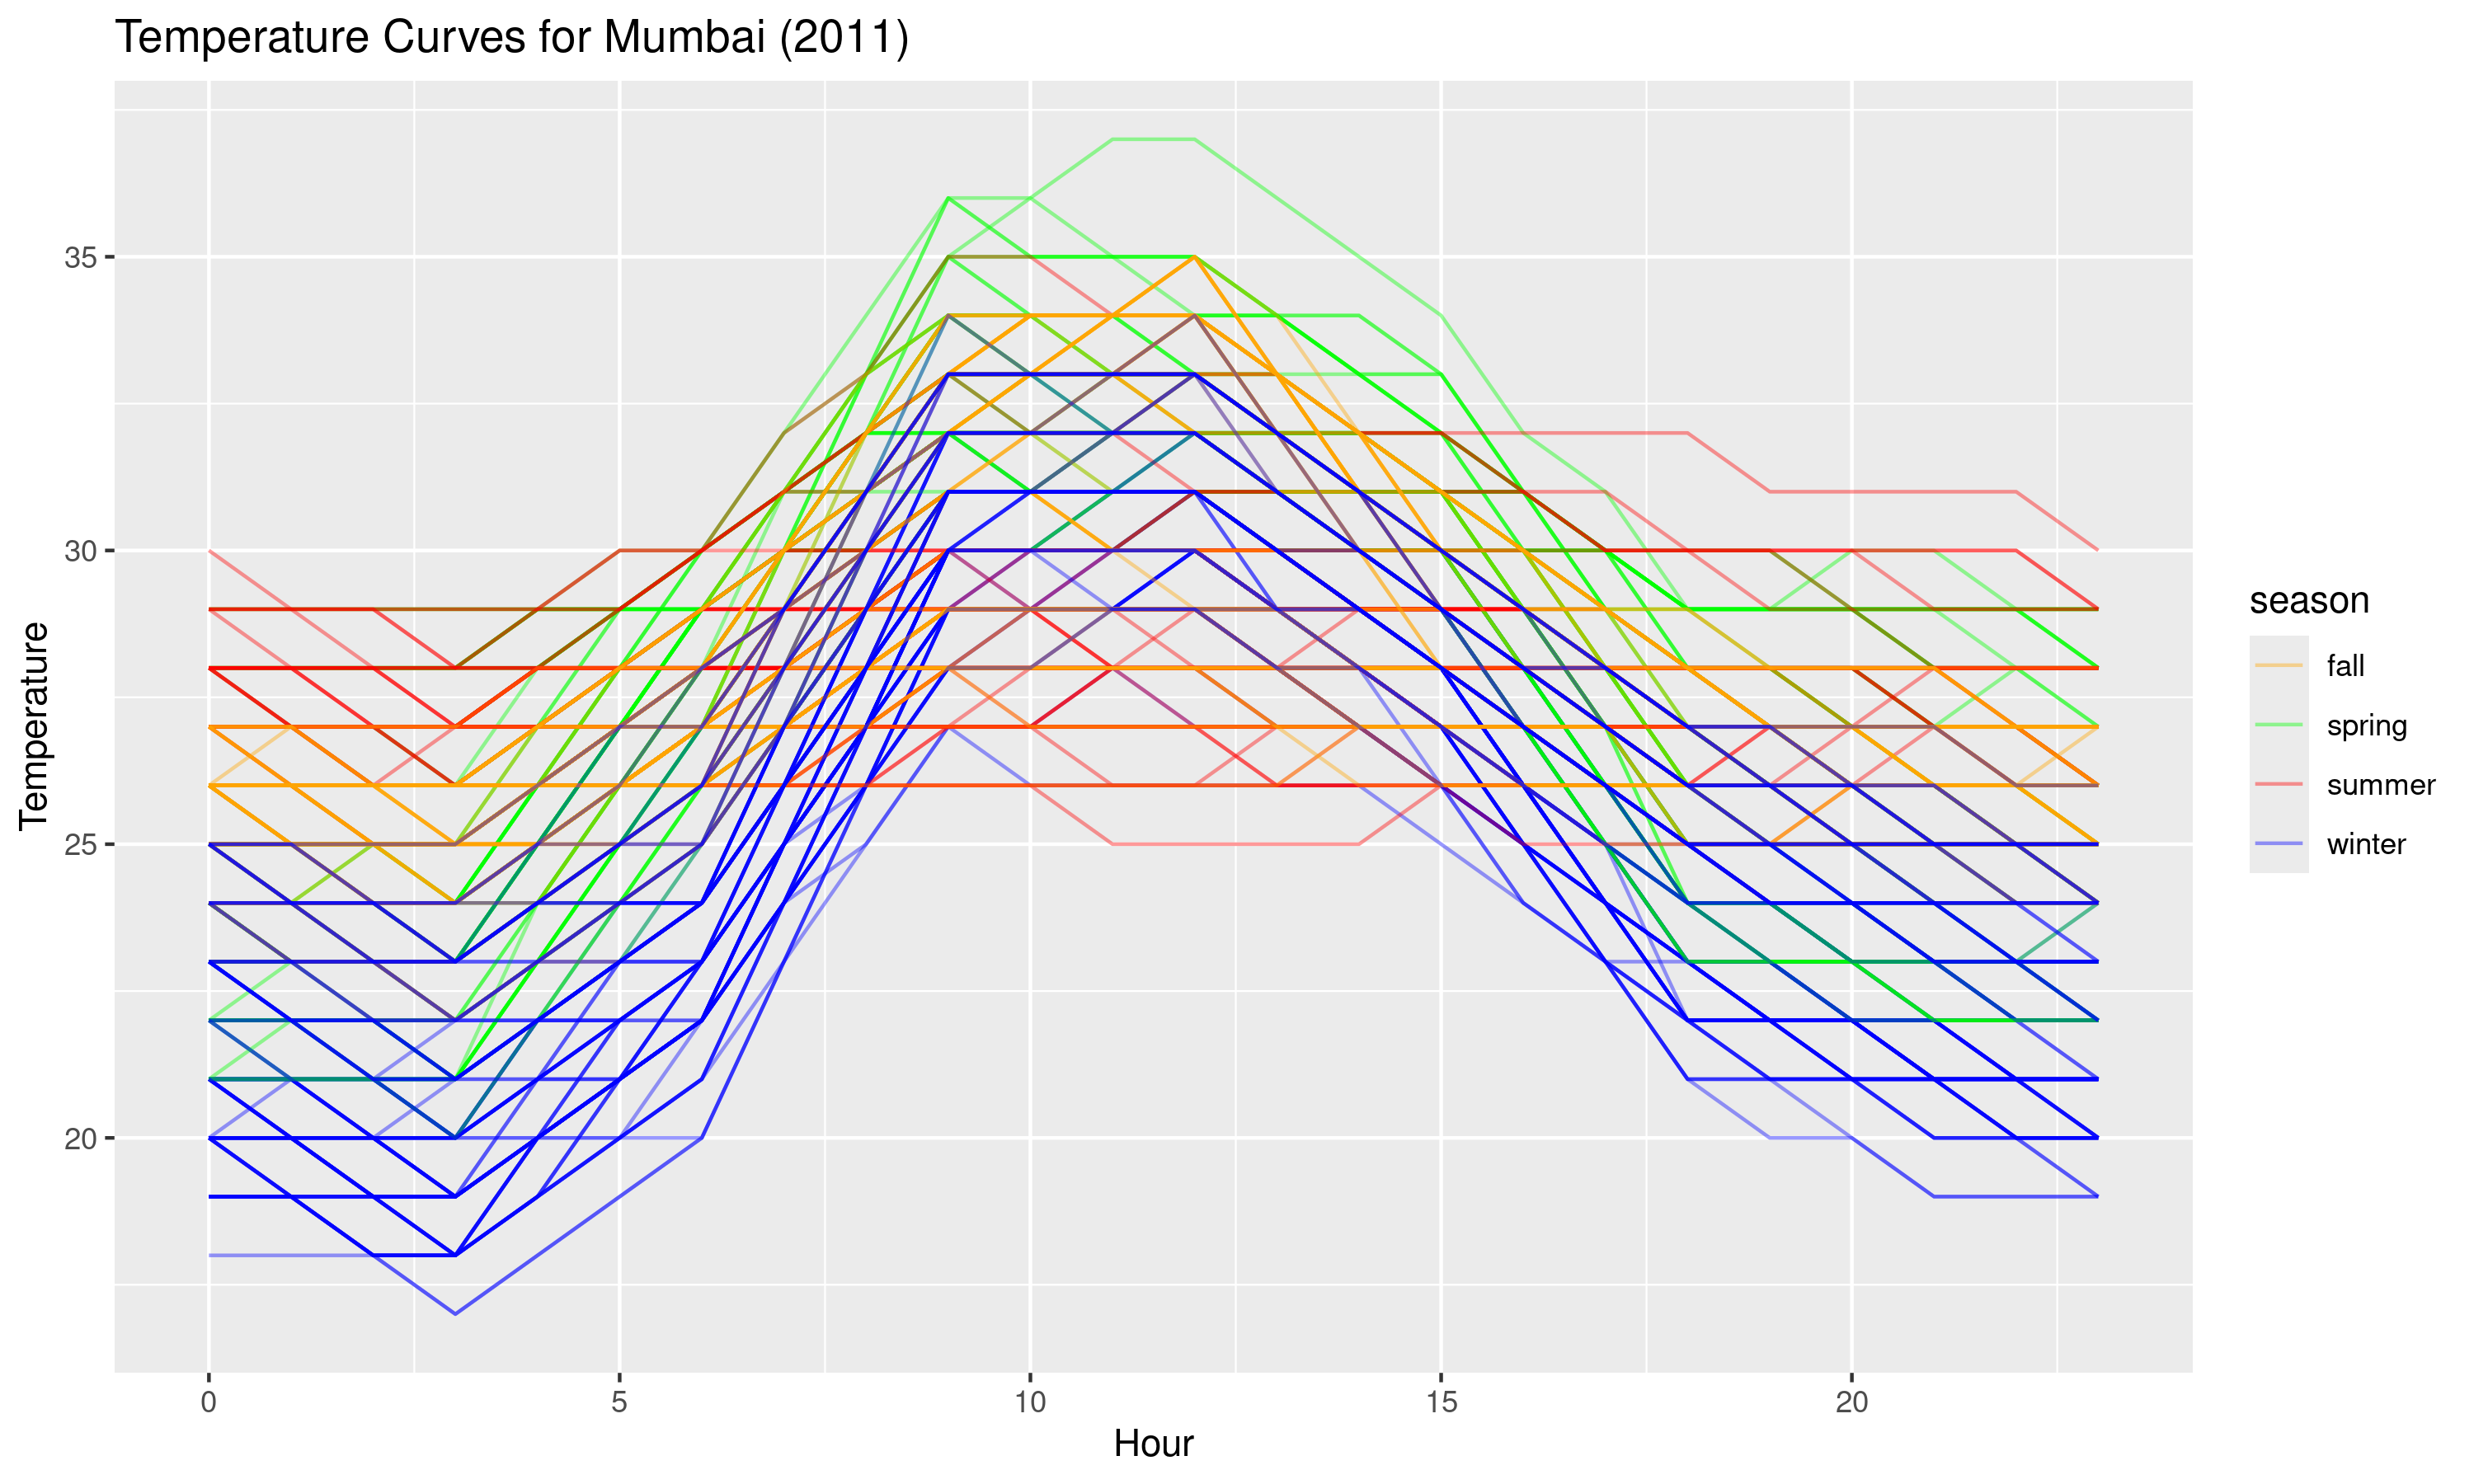
\includegraphics[width=0.8\linewidth]{../notebooks/assets/unsmoothed_temperature_curves.png}
	\end{center}
\end{frame}

\begin{frame}{Lambda Search: Smoothing Parameter Tuning}
    \begin{itemize}
        \item Looking for the optimal smoothing parameter \(\lambda\).
		\item GCV evaluated for \(\lambda\) values from \(10^{-4}\) to \(10^{0.6}\).
    \end{itemize}
    \vfill
    \begin{center}
        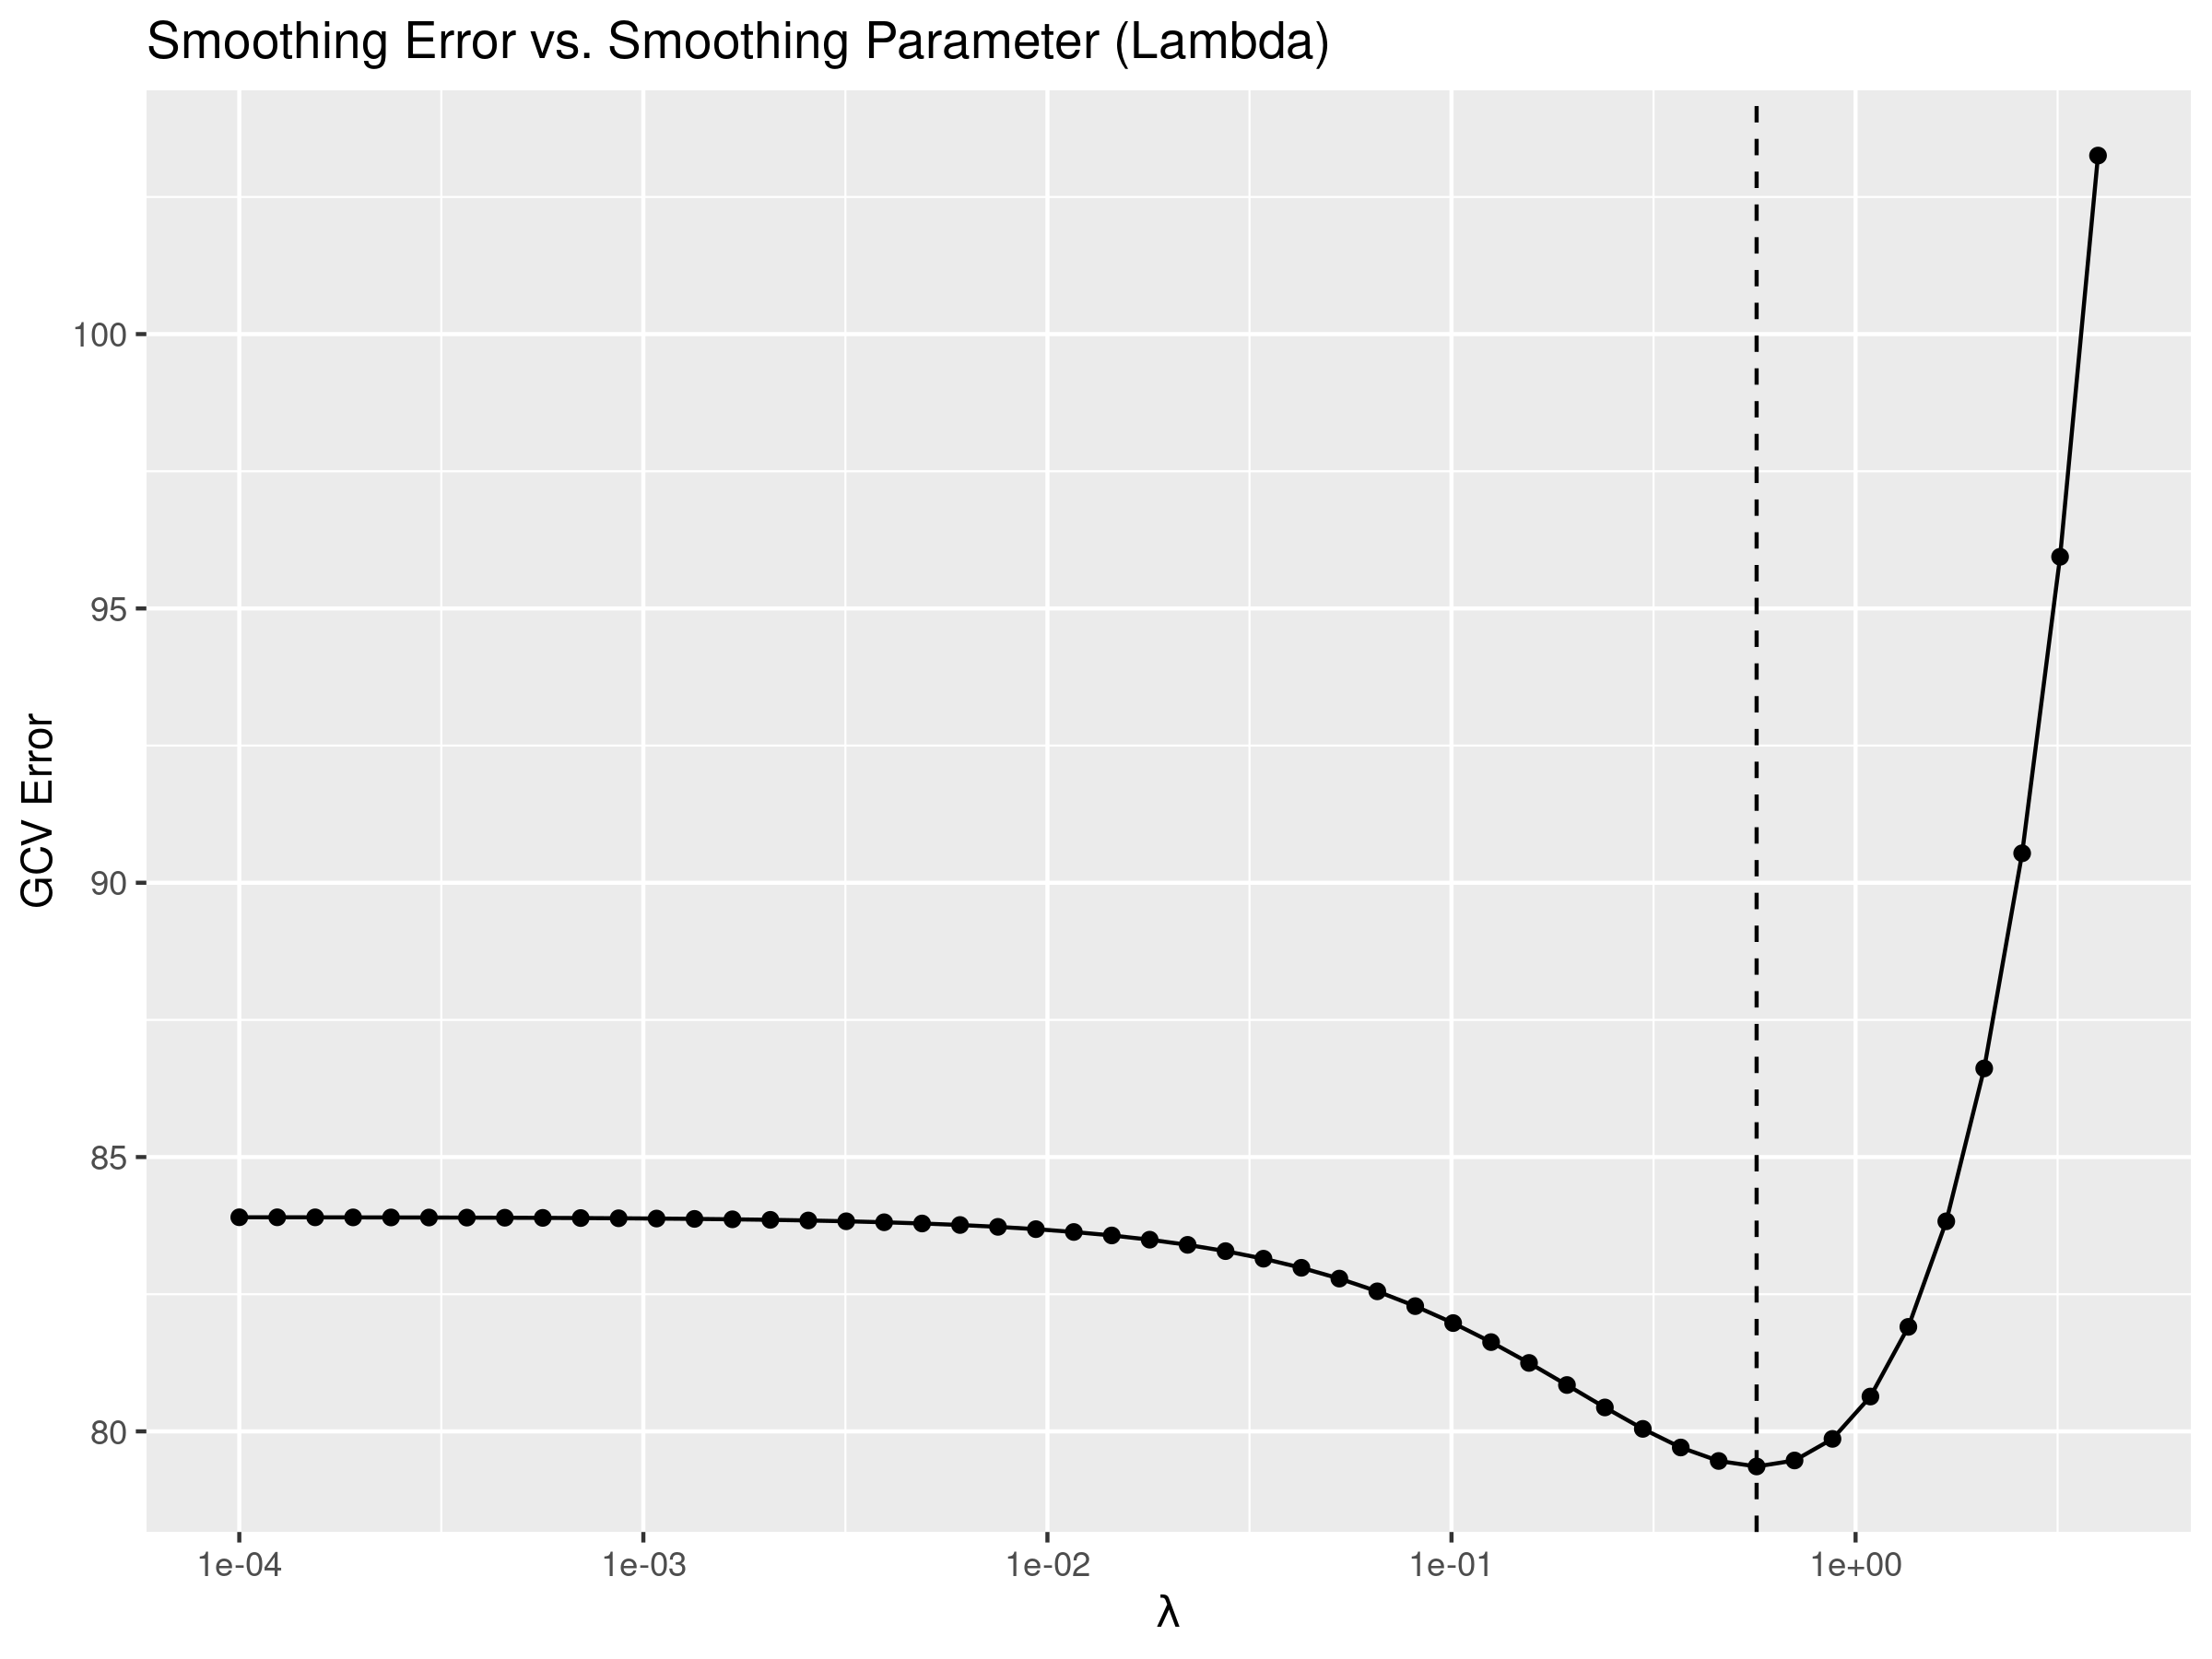
\includegraphics[width=0.7\linewidth]{../notebooks/assets/lambda_vs_gcv.png}
    \end{center}
\end{frame}

\begin{frame}{Smoothed Temperature Curves}
		\begin{itemize}
		\item Applied B-spline smoothing (8 basis functions, $\lambda=0.5$).
		\item Smoothed curves reveal underlying daily patterns.
	\end{itemize}
	\begin{center}
		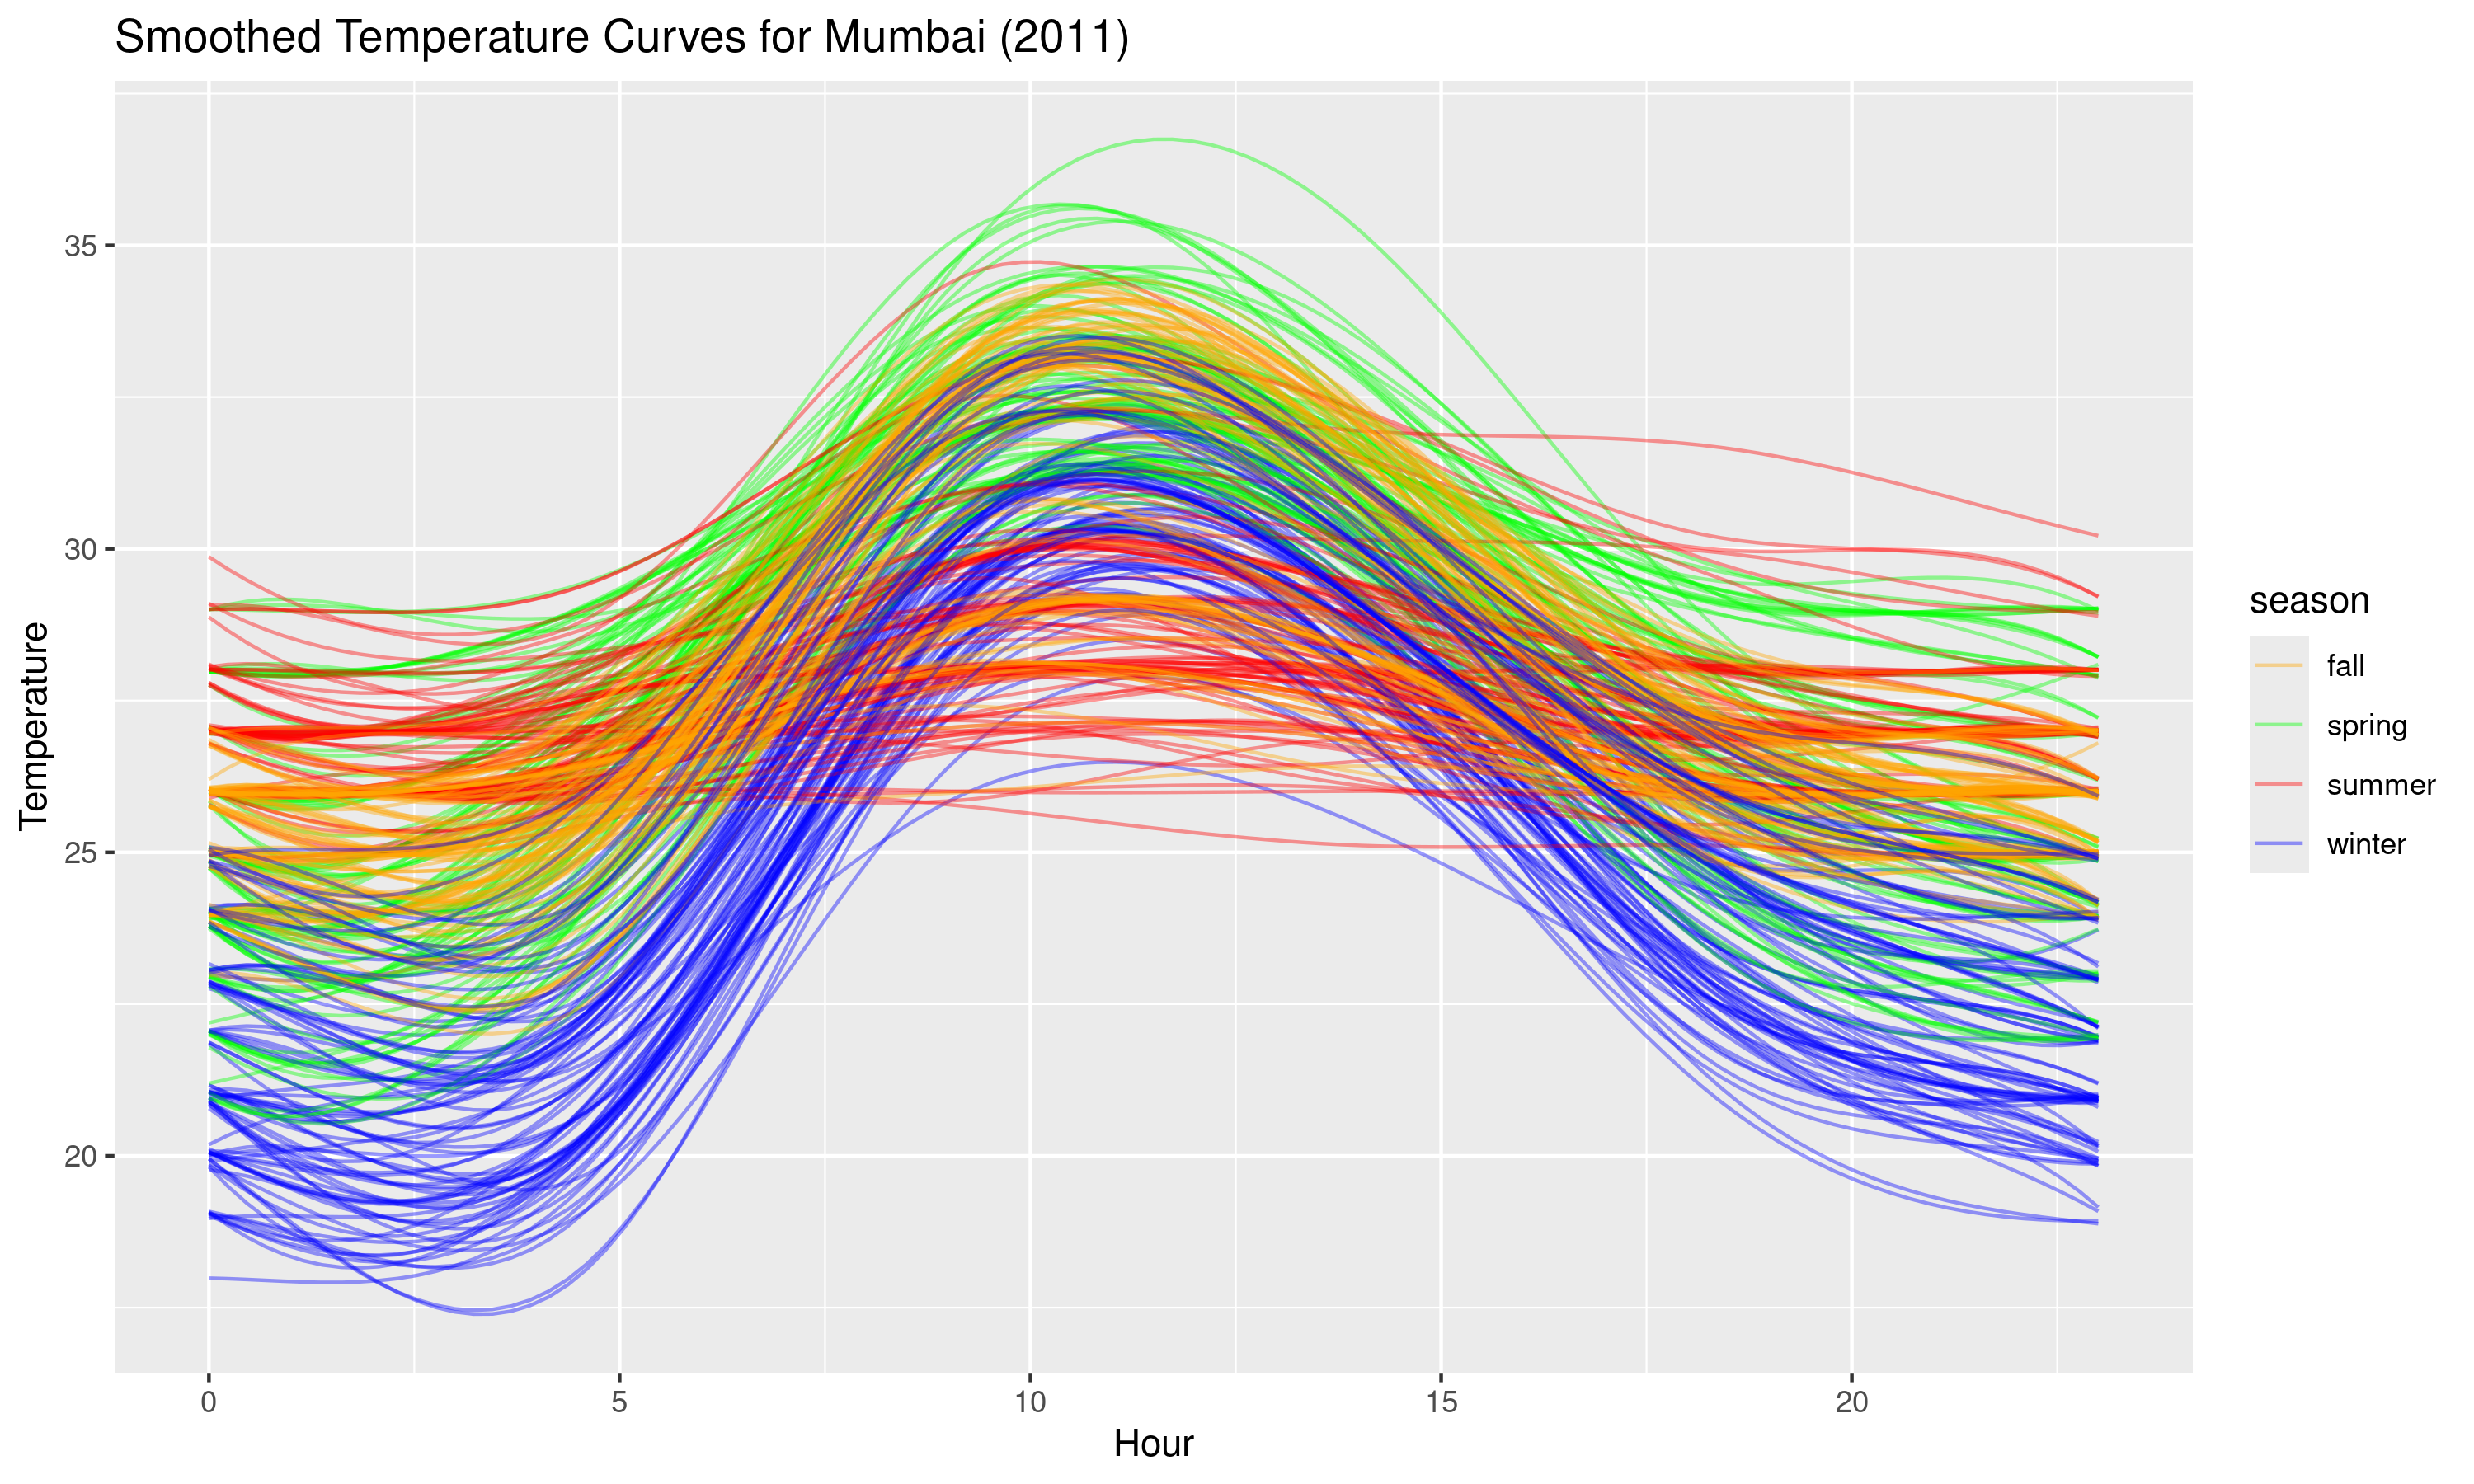
\includegraphics[width=0.8\linewidth]{../notebooks/assets/smoothed_temperature_curves.png}
	\end{center}
\end{frame}

\section{Derivatives \& Covariance}

\begin{frame}{Derivative Analysis}
	\begin{itemize}
		\item Computed first derivative (slope) and second derivative (acceleration) of the smoothed curves.
		\item Noted boundary effects with extreme derivative values at t = 0 and t = 23.
		\end{itemize}
	\begin{center}
		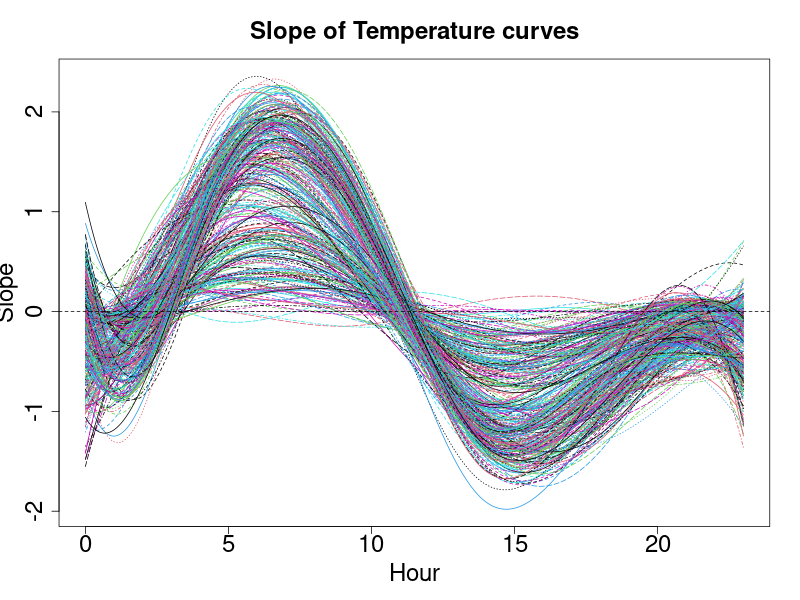
\includegraphics[width=0.48\linewidth]{../notebooks/assets/slope_fd_plot.png}\hfill
		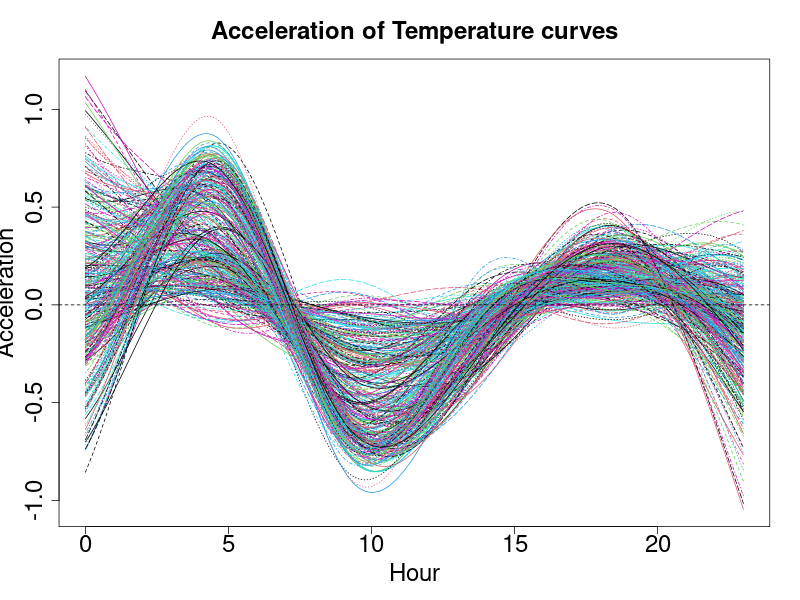
\includegraphics[width=0.48\linewidth]{../notebooks/assets/acceleration_fd_plot.png}
	\end{center}
\end{frame}

\begin{frame}{Covariance Analysis}
		\begin{itemize}
		\item Estimated the covariance function from the smoothed functional data.
		\item Visualized as a 2D heatmap to assess variability over the day.
	\end{itemize}
	\begin{center}
		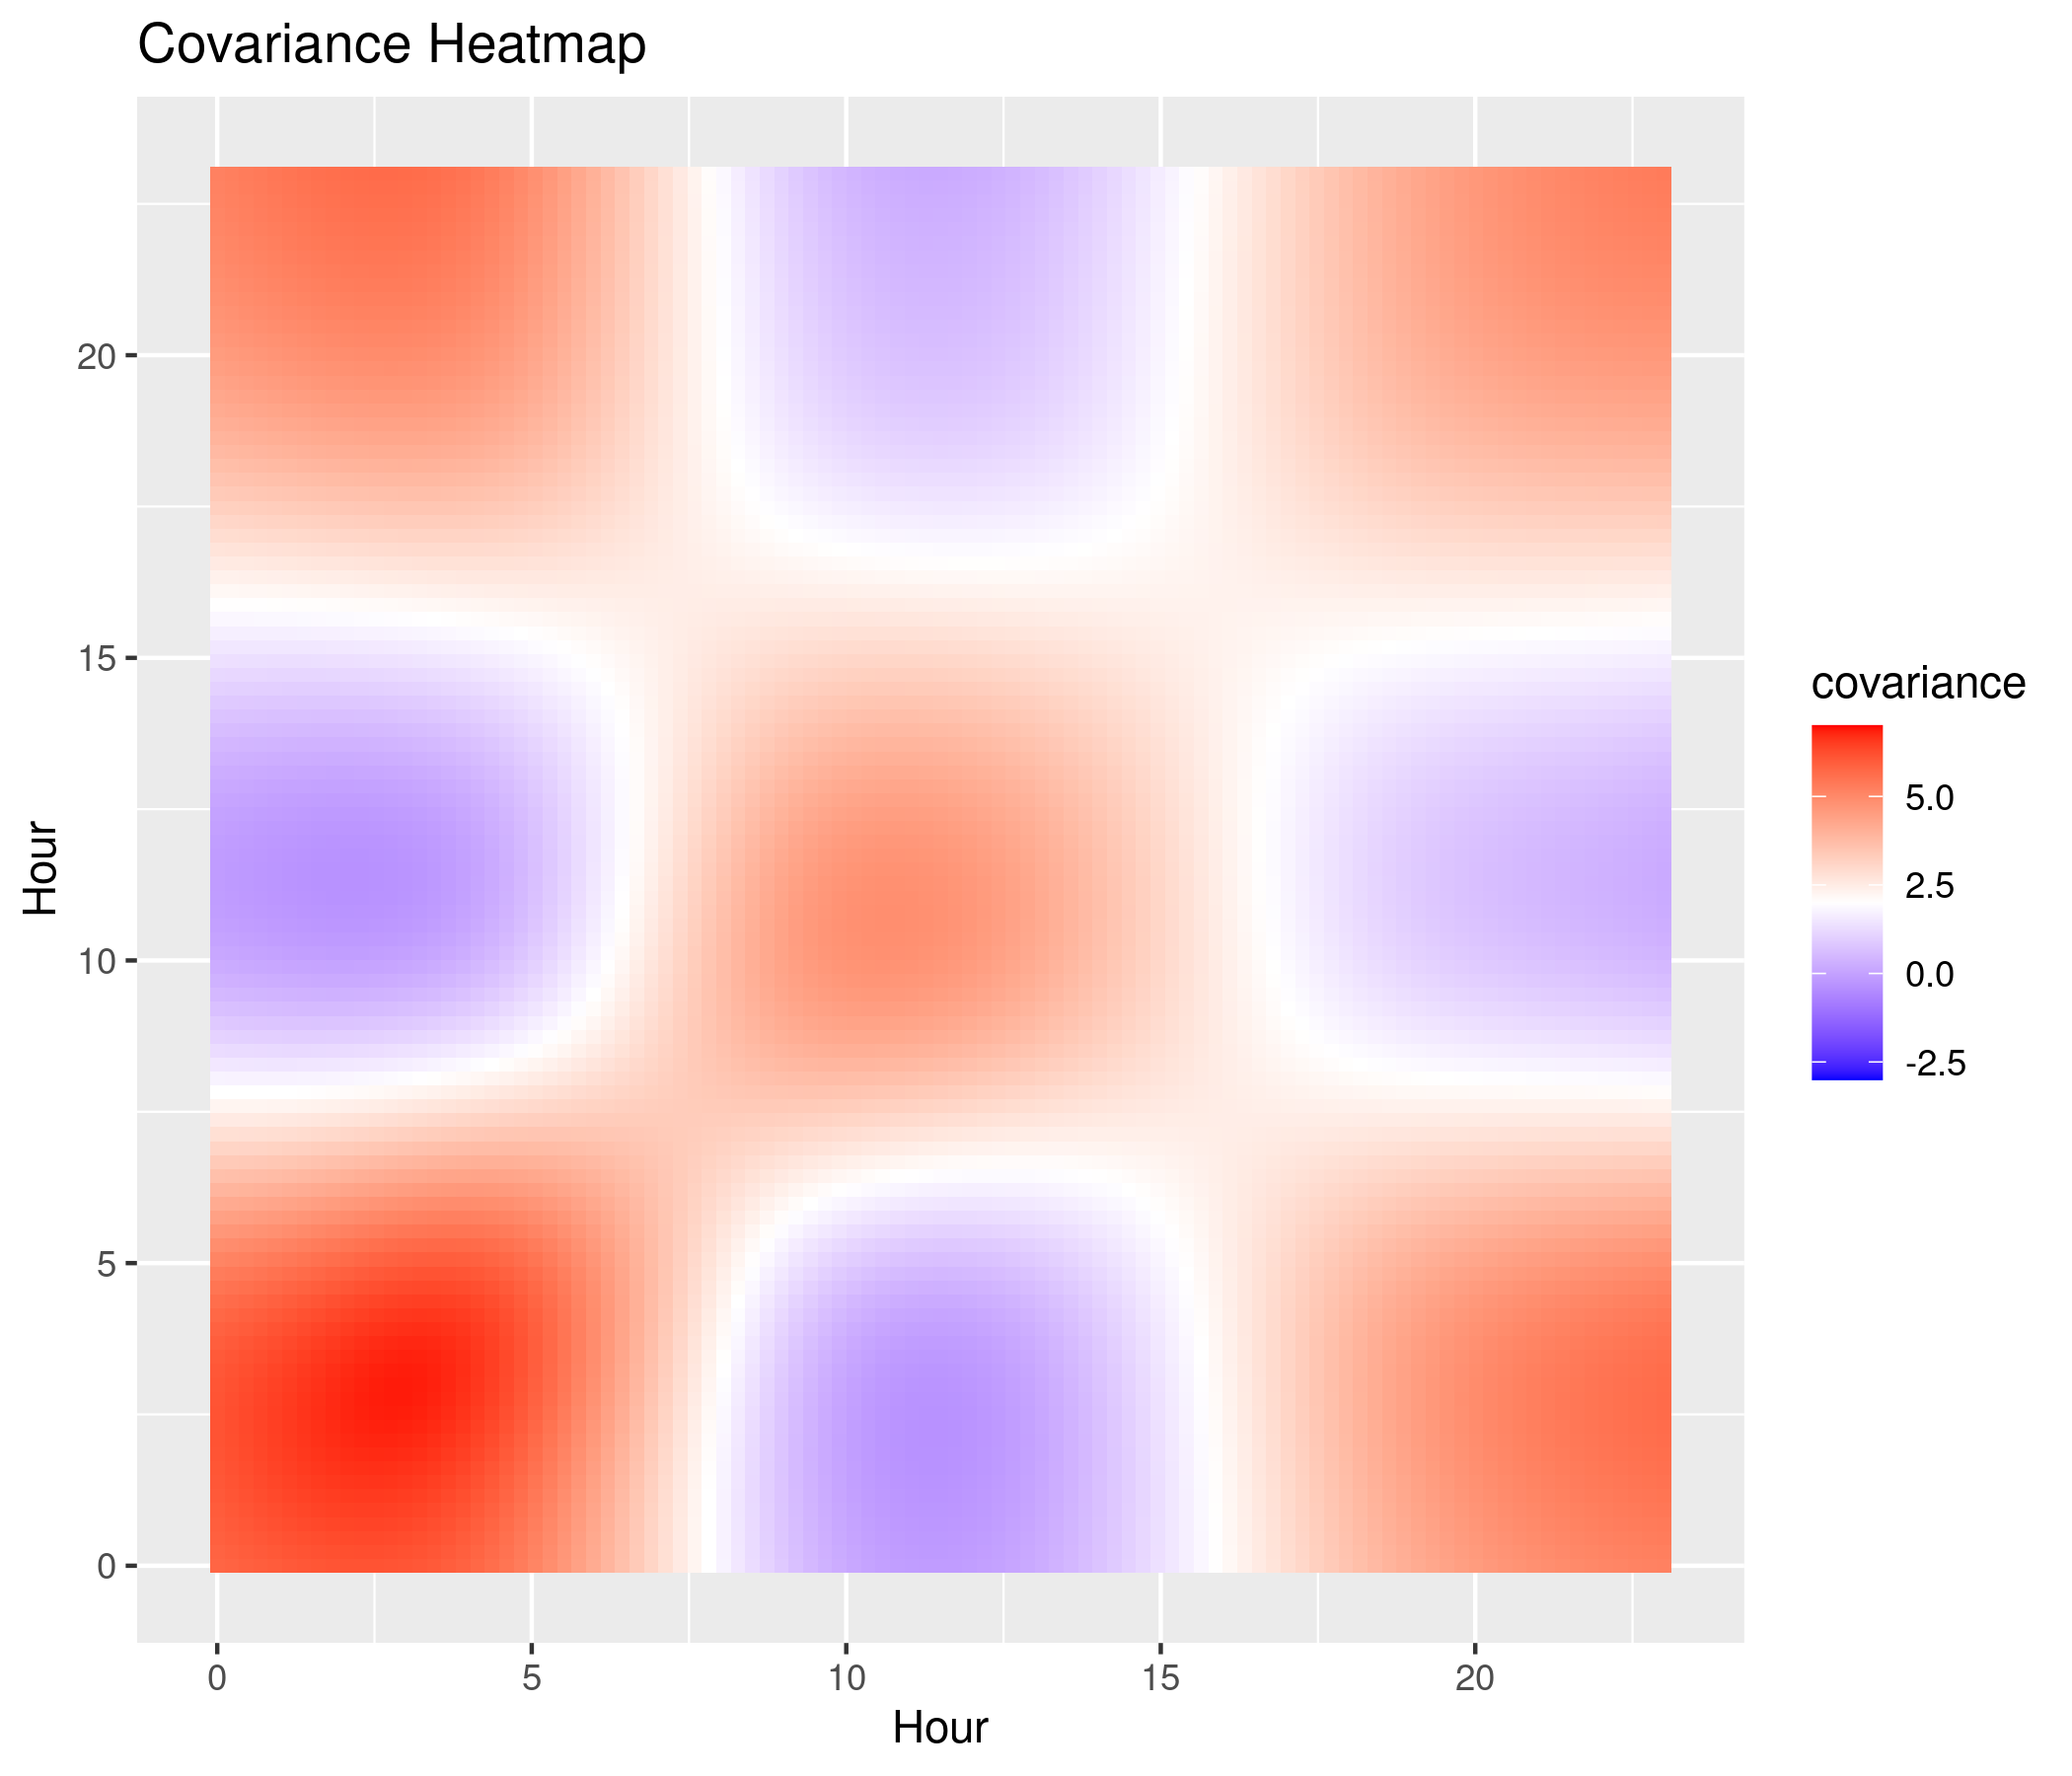
\includegraphics[width=0.6\linewidth]{../notebooks/assets/covariance_heatmap.png}
	\end{center}
\end{frame}

\section{FPCA}

\begin{frame}{Functional Principal Component Analysis (FPCA)}
	\begin{itemize}
		\item Performed FPCA on the smoothed temperature curves.
		\item Extracted the first 3 principal components.
	\end{itemize}
	\begin{center}
		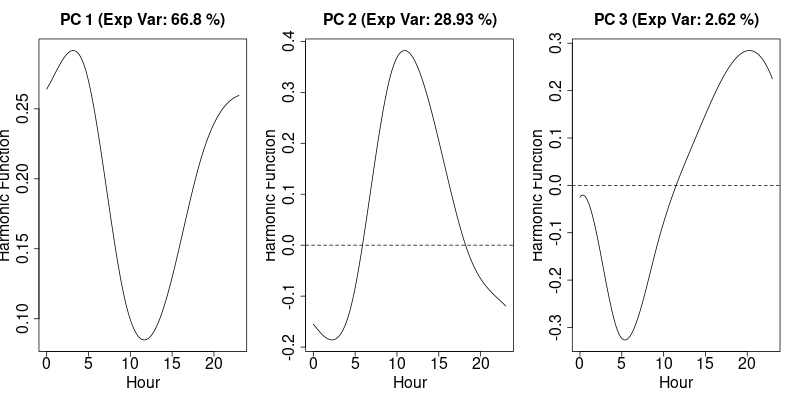
\includegraphics[width=0.8\linewidth]{../notebooks/assets/pca_scree_plot.png}
	\end{center}
\end{frame}

\section{Summary \& Future Work}

\begin{frame}{Summary \& Future Work}
	\begin{itemize}
		\item \textbf{Key findings:}
		\begin{itemize}
			\item FDA can reveal daily patterns in temperature data.
		\end{itemize}
		\item \textbf{Future directions:}
		\begin{itemize}
			\item Decide on the direction of the analysis (daily vs yearly patterns, possibly use more cities).
			\item Continue exploring the data with more advanced FDA techniques.
		\end{itemize}
	\end{itemize}
\end{frame}

\end{document}
